\documentclass[12pt,a4paper]{article}

% --------------------------------------------------
% Packages
% --------------------------------------------------
\usepackage[
    a4paper,
    top=25mm,
    bottom=25mm,
    left=25mm,
    right=25mm
]{geometry}

\usepackage{graphicx}
\usepackage{booktabs}
\usepackage{longtable}
\usepackage{array}
\usepackage{amsmath}
\usepackage{amssymb}
\usepackage{microtype}
\usepackage{multirow}
\usepackage{rotating}
\usepackage[table]{xcolor}
\usepackage{hyperref}

% --------------------------------------------------
% Hyperref setup
% --------------------------------------------------
\hypersetup{
    colorlinks=true,
    linkcolor=black,
    urlcolor=blue,
    pdftitle={PartnerAPI - Audited Documentation Addendum},
    pdfauthor={Software Engineering Project}
}

% --------------------------------------------------
% Document formatting
% --------------------------------------------------
\setlength{\parindent}{0pt}
\setlength{\parskip}{8pt}
\renewcommand{\arraystretch}{1.2}
\emergencystretch=3em

% --------------------------------------------------
% Title
% --------------------------------------------------
\title{
    \textbf{PartnerAPI}\\[6pt]
    \large Audited Documentation Addendum
}

\author{Software Engineering Project}
\date{\today}

% --------------------------------------------------
% Document
% --------------------------------------------------
\begin{document}

\maketitle

\tableofcontents

\newpage

% ==================================================
\section{Introduction}
% ==================================================

This document serves as the formal addendum to the PartnerAPI project
documentation suite. It supplements the original documents by
providing the explicitly required visual diagrams and computed
mathematical evidence for testing and risk management as highlighted
during the documentation audit.

% ==================================================
\section{Testing Addendum (Supplement to Test Plan)}
% ==================================================

% --------------------------------------------------
\subsection{Defect Log}
% --------------------------------------------------

Table~\ref{tab:defect-log} provides the aggregated defect counts
identified during the initial testing phases of PartnerAPI.

\begin{table}[htbp]
    \centering

    \begin{tabular}{lr}
        \toprule
        \textbf{Metric} & \textbf{Count} \\
        \midrule

        Defects found before release ($D_{\text{before}}$)
        & 25 \\

        Defects found after release ($D_{\text{after}}$)
        & 2 \\

        \midrule

        \textbf{Total Defects Identified ($D_{\text{total}}$)}
        & \textbf{27} \\

        \bottomrule
    \end{tabular}

    \caption{PartnerAPI Summary Defect Log}
    \label{tab:defect-log}
\end{table}

% --------------------------------------------------
\subsection{Defect Density Computation}
% --------------------------------------------------

Defect Density measures the number of defects relative to the size
of the software.

For PartnerAPI, the software size is evaluated at 10 KLOC
(Thousands of Lines of Code).

\[
\text{Defect Density}
=
\frac{\text{Total Defects}}
{\text{Software Size (KLOC)}}
\]

Therefore:

\[
\text{Defect Density}
=
\frac{27}{10}
=
\mathbf{2.7\text{ defects per KLOC}}
\]

% --------------------------------------------------
\subsection{Defect Removal Efficiency (DRE)}
% --------------------------------------------------

Defect Removal Efficiency determines the percentage of defects
successfully caught prior to production release.

\[
\text{DRE}
=
\left(
\frac{D_{\text{before}}}
{D_{\text{before}} + D_{\text{after}}}
\right)
\times 100
\]

Therefore:

\[
\text{DRE}
=
\left(
\frac{25}{25+2}
\right)
\times 100
\]

\[
\text{DRE}
=
\frac{25}{27}
\times 100
=
\mathbf{92.59\%}
\]

A DRE of 92.59\% indicates that the majority of identified defects
were detected before production release.

\newpage

% ==================================================
\section{Project Plan Addendum}
% ==================================================

% --------------------------------------------------
\subsection{Network Diagram (PERT)}
% --------------------------------------------------

The network diagram below illustrates the sequential critical path
of the standard baseline release. Custom partner requests are
excluded from this baseline path.

\begin{figure}[htbp]
    \centering
    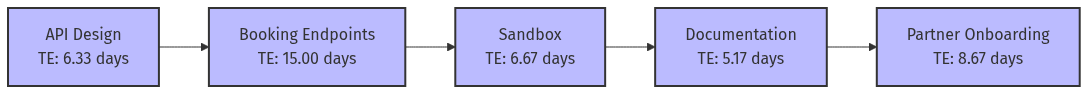
\includegraphics[
        width=\textwidth,
        height=0.65\textheight,
        keepaspectratio
    ]{../diagrams/network/network.png}

    \caption{PartnerAPI Network Diagram (Critical Path)}
    \label{fig:network-diagram}
\end{figure}

% --------------------------------------------------
\subsection{Gantt Chart}
% --------------------------------------------------

The Gantt chart visually maps the schedule timeline against the
three-point Expected Time (TE) values calculated in the Estimation
Sheet.

\begin{figure}[htbp]
    \centering
    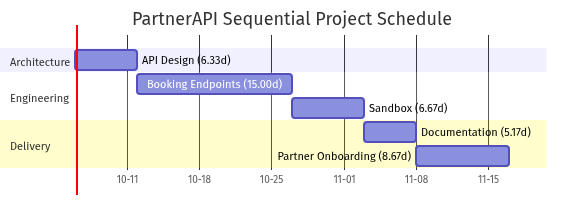
\includegraphics[
        width=\textwidth,
        height=0.65\textheight,
        keepaspectratio
    ]{../diagrams/gantt/gantt.png}

    \caption{PartnerAPI Baseline Gantt Chart}
    \label{fig:gantt-chart}
\end{figure}

\newpage

% ==================================================
\section{Risk Register Addendum}
% ==================================================

% --------------------------------------------------
\subsection{Probability-Impact Matrix}
% --------------------------------------------------

Table~\ref{tab:risk-matrix} visualizes the standard
Probability-Impact Matrix utilized to assess Risk Exposure for
PartnerAPI.

The risks R1 through R5 from the Risk Register are plotted according
to their assessed severity.

\begin{table}[htbp]
    \centering

    \renewcommand{\arraystretch}{2}

    \begin{tabular}{|c|p{2.5cm}|c|c|c|}
        \hline

        \multicolumn{2}{|c|}{}
        &
        \multicolumn{3}{c|}{\textbf{Impact}}
        \\

        \cline{3-5}

        \multicolumn{2}{|c|}{}
        &
        \textbf{Low}
        &
        \textbf{Medium}
        &
        \textbf{High}
        \\

        \hline

        \multirow{3}{*}{
            \rotatebox{90}{\textbf{Probability}}
        }
        &
        \textbf{High}
        &
        &
        &
        \cellcolor{red!30}
        \textbf{R1, R3}
        \\

        \cline{2-5}

        &
        \textbf{Medium}
        &
        &
        \cellcolor{yellow!30}
        \textbf{R5}
        &
        \cellcolor{red!30}
        \textbf{R2}
        \\

        \cline{2-5}

        &
        \textbf{Low}
        &
        &
        &
        \cellcolor{red!30}
        \textbf{R4}
        \\

        \hline
    \end{tabular}

    \vspace{0.5cm}

    \caption{PartnerAPI Probability-Impact Matrix}
    \label{tab:risk-matrix}
\end{table}

\vspace{0.5cm}

\noindent\textbf{Legend:}

\begin{itemize}
    \item \textbf{R1}: Internal booking-system integration delay
    (High/High).

    \item \textbf{R2}: Partner integration problems
    (Medium/High).

    \item \textbf{R3}: Scope expansion through custom requests
    (High/High).

    \item \textbf{R4}: Security vulnerability
    (Low/Very High, mapped to High for the standard grid).

    \item \textbf{R5}: Documentation delay
    (Medium/Medium).
\end{itemize}

% ==================================================
\section{Summary}
% ==================================================

The audited addendum provides additional quantitative and visual
evidence supporting the PartnerAPI project documentation.

The testing evidence records 27 identified defects, consisting of
25 defects found before release and 2 defects found after release.
This results in a defect density of 2.7 defects per KLOC and a
Defect Removal Efficiency of 92.59\%.

The network diagram and Gantt chart provide visual evidence of the
baseline project schedule, while the Probability-Impact Matrix
summarises the assessed project risks.

These additions complement the existing Test Plan, Project Plan and
Risk Register documentation.

\end{document}

